\section{Intel RAPL Leakage Analysis}
Intel Software Guard Extensions (SGX) is an architectural extension of x86 processors
designed to provide secure, isolated execution environments known as enclaves. Enclaves
are regions of application memory where code and data are protected by hardware from
all other software on the system, including the operating system, hypervisor, and even the
system BIOS. The core security guarantee is that even if the rest of the platform is fully
compromised, enclave memory contents remain confidential and tamper-resistant.
When a process creates an enclave, the memory pages assigned to it are designated as
special by the SGX hardware. Accesses to this range are permitted only during enclave
mode; any access attempt by non-enclave code, regardless of privilege level, is blocked.
This is enforced by checks at the CPU’s memory controller, effectively preventing even
kernel or DMA attacks. 
\begin{figure}
    \centering
    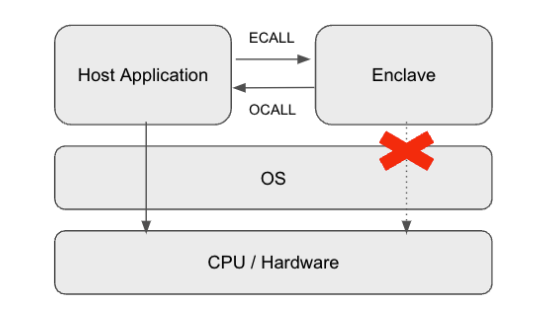
\includegraphics[width=0.8\linewidth]{Assignment2- Writing a Research Paper in Latex/Images/Intel_SGX.png}
    \caption{Organization of Intel SGX}
    \label{fig:Intel_SGX}
\end{figure}
Organization of protected memory regions in Intel SGX is shown in Figure \ref{fig:Intel_SGX}. Enclave code and data are inaccessible to the OS and all other non-enclave software.